\let\negmedspace\undefined
\let\negthickspace\undefined
\documentclass[journal]{IEEEtran}
\usepackage[a5paper, margin=10mm, onecolumn]{geometry}
\usepackage{lmodern} % Ensure lmodern is loaded for pdflatex
\usepackage{tfrupee} % Include tfrupee package

\setlength{\headheight}{1cm} % Set the height of the header box
\setlength{\headsep}{0mm}     % Set the distance between the header box and the top of the text

\usepackage{gvv-book}
\usepackage{gvv}
\usepackage{cite}
\usepackage{amsmath,amssymb,amsfonts,amsthm}
\usepackage{algorithmic}
\usepackage{graphicx}
\usepackage{textcomp}
\usepackage{xcolor}
\usepackage{txfonts}
\usepackage{listings}
\usepackage{enumitem}
\usepackage{mathtools}
\usepackage{gensymb}
\usepackage{comment}
\usepackage[breaklinks=true]{hyperref}
\usepackage{tkz-euclide} 
\usepackage{listings}
\usepackage{gvv}                                        
\def\inputGnumericTable{}                                 
\usepackage[latin1]{inputenc}                                
\usepackage{color}                                            
\usepackage{array}                                            
\usepackage{longtable}                                       
\usepackage{calc}                                             
\usepackage{multirow}                                         
\usepackage{hhline}                                           
\usepackage{ifthen}                                           
\usepackage{lscape}
\begin{document}

\bibliographystyle{IEEEtran}
\vspace{3cm}

\title{10.4.ex.12}
\author{EE24BTECH11060-Sruthi bijili}
% \maketitle
% \newpage
% \bigskip
{\let\newpage\relax\maketitle}
\textbf{Question:}\\
A rectangular park is to be designed whose breadth is $3$ m less than its length. Its area is to be $4$ square metres more than the area of a park that has already been made in the shape of an isosceles triangle with its base as the breadth of the rectangular park and of altitude $12$ m . Find its length and breadth.\\
\textbf{Solution:}\\
Let the length of the park is $x+3$ and breadth is $x$.\\
Given that the altitude of triangle is $12m$\\ 
Area of the isosceles triangle =$\frac{1}{2}\brak{x}12$\\
Given that area of the rectangle is = 4+area of triangle\\
Area of the rectangle = $x\brak{x+3}$\\
\textbf{Theoretical solution:}
According to the question:\\
\begin{align}
    \implies x\brak{x+3}=4+6x
    \implies x^2-3x-4=0
\end{align}
Applying the quadratic formula,we get
\begin{align}
    x_1=\frac{3+\sqrt{9-4\brak{-4}}}{2}\\
    x_1=\frac{3+\sqrt{25}}{2}\\
    x_1=4\\
    x_2=\frac{3-\sqrt{9-\brak{-4}}}{2}\\
    x_2=\frac{3-\sqrt{25}}{2}\\
    x_2=-1
\end{align}
Therefore, the breadth of the rectangle is $4$m and length is $7$m\\
\textbf{Computational Solution:}
\subsection*{ Newton-Raphson Method}
The Newton-Raphson method is defined as:
\begin{align}
    x_{n+1} = x_n - \frac{f(x_n)}{f'(x_n)}
\end{align}
Here:
\begin{align}
    f(x) = x^2 - 3x - 4, \quad f'(x) = 2x - 3
\end{align}
Substitute into the formula:
\begin{align}
    x_{n+1} = x_n - \frac{x_n^2 - 3x_n - 4}{2x_n - 3}
\end{align}
The problem with this method is if the roots are complex but the coeffcients are real, $x_n$ either converges to an extrema or grows continuously without any bound.
	To get the complex solutions, however, we can just take the initial guess point to be a 
	random complex number.\\

\textbf{Starting with an initial guess \( x_0 = 3 \):}
\begin{align}
    x_1 = 3 - \frac{3^2 - 3(3) - 4}{2(3) - 3} = 3 - \frac{9 - 9 - 4}{6 - 3} = 3 + \frac{4}{3} \approx 4.33 \\
    x_2 = 4.33 - \frac{4.33^2 - 3(4.33) - 4}{2(4.33) - 3} \approx 4.02
\end{align}
The same for the other root the output of a program written to find roots is shown below:
	\begin{align}
		x_1 = 4\\
		x_2 = -1\\
	\end{align}

\section*{Companion Matrix}
For a quadratic equation of the form:
\begin{align}
    ax^2 + bx + c = 0,
\end{align}
the corresponding companion matrix is given by:
\begin{align}
    A = 
    \myvec{
        0 & 1 \\
        -\frac{c}{a} & -\frac{b}{a}
    }.
\end{align}

Substitute the coefficients $a = 1$, $b = -3$, ad $c = -4$ into the companion matrix formula:
\begin{align}
    A = 
    \myvec{
        0 & 1 \\
        3 & 4
    }
\end{align}

\section*{QR Algorithm}
The QR algorithm iteratively decomposes the matrix $A_n$ into an orthogonal matrix $Q_n$ and an upper triangular matrix $R_n$, and updates the matrix as:
\begin{align}
    A_{n+1} = R_n Q_n.
\end{align}
This process continues until $A_n$ converges to an upper triangular matrix, where the diagonal elements are the eigenvalues of $A$.

\subsection*{Steps of the Algorithm}
\begin{enumerate}
    \item Initialize the companion matrix:
    \begin{align}
        A_0 = 
        \myvec{
            0 & 1 \\
            3 & 4
        }.
    \end{align}
    \item Perform QR decomposition of $A_n$:
    \begin{align}
        A_n = Q_n R_n,
    \end{align}
    where $Q_n$ is orthogonal and $R_n$ is upper triangular.
    \item Update the matrix:
    \begin{align}
        A_{n+1} = R_n Q_n.
    \end{align}
    \item Repeat the above steps until $A_n$ converges to an upper triangular matrix. The diagonal elements of this matrix are the eigenvalues, which correspond to the roots of the quadratic equation.
\end{enumerate}

\subsection*{Roots of the Quadratic Equation}
The eigenvalues of the companion matrix $A$ are the roots of the quadratic equation. Applying the QR algorithm numerically to $A$, we find:
\begin{align}
    \lambda_1 = 4, \quad \lambda_2 = -1
\end{align}

\subsection*{Conclusion}
The QR decomposition method applied to the companion matrix of $x^2-3x-4= 0$ finds the roots of the equation. Both roots are real and distinct:
\begin{align}
    x_1 =4,x_2=-1
\end{align}
This demonstrates the utility of the QR algorithm in computing eigenvalues, which are the roots of polynomial equations.
Below is the plot for line and the parabola
\begin{figure}[h!]
	\centering
	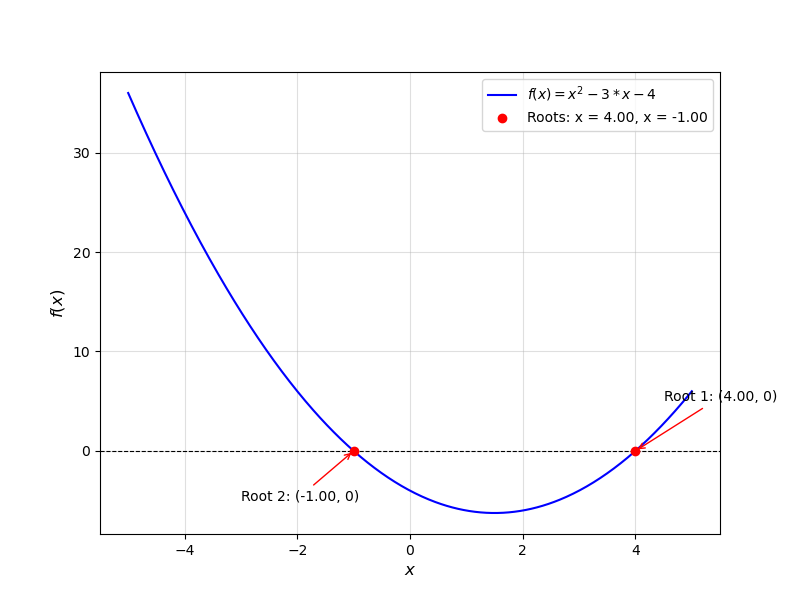
\includegraphics[width=1\columnwidth]{figs/fig.png}
	\label{stemplot}
\end{figure}





\end{document}
